\documentclass[11pt,compress,t,notes=noshow, aspectratio=169, xcolor=table]{beamer}
\newcommand{\btVFill}{\vskip0pt plus 1filll}
\newcommand\hmmax{0}
\newcommand\bmmax{0}
\usepackage{../../style/lmu-lecture}
\usepackage{siunitx}
% Defines macros and environments
% This file is included in slides and exercises

% Rarely used fontstyle for R packages, used only in 
% - forests/slides-forests-benchmark.tex
% - exercises/single-exercises/methods_l_1.Rnw
% - slides/cart/attic/slides_extra_trees.Rnw
\newcommand{\pkg}[1]{{\fontseries{b}\selectfont #1}}

% Spacing helpers, used often (mostly in exercises for \dlz)
\newcommand{\lz}{\vspace{0.5cm}} % vertical space (used often in slides)
\newcommand{\dlz}{\vspace{1cm}}  % double vertical space (used often in exercises, never in slides)
\newcommand{\oneliner}[1] % Oneliner for important statements, used e.g. in iml, algods
{\begin{block}{}\begin{center}\begin{Large}#1\end{Large}\end{center}\end{block}}

% Don't know if this is used or needed, remove?
% textcolor that works in mathmode
% https://tex.stackexchange.com/a/261480
% Used e.g. in forests/slides-forests-bagging.tex
% [...] \textcolor{blue}{\tfrac{1}{M}\sum^M_{m} [...]
% \makeatletter
% \renewcommand*{\@textcolor}[3]{%
%   \protect\leavevmode
%   \begingroup
%     \color#1{#2}#3%
%   \endgroup
% }
% \makeatother


\title{Interpretable Machine Learning}
% \author{LMU}
%\institute{\href{https://compstat-lmu.github.io/lecture_iml/}{compstat-lmu.github.io/lecture\_iml}}
\date{}

\begin{document}

% TODO
\newcommand{\titlefigure}{figure_man/exSHAP.png}
% \newcommand{\learninggoals}{
% \item Get an intuition of additive feature attributions
% \item Understand the concept of Kernel SHAP
% \item Ability to interpret SHAP plots
% \item Global SHAP methods
% }
\newcommand{\learninggoals}{
\item Understand KernelSHAP as weighted least-squares regression over coalitions
\item Grasp how background samples impute "absent" features
\item Observational vs. interventional SHAP
}

\lecturechapter{SHAP (SHapley Additive exPlanation) Values}
\lecture{Interpretable Machine Learning}

%\begin{frame}{Example}

%Given the following example from the bike sharing data set

%\begin{table}[h]
%\centering
%\begin{tabular}{l rrrrr || r}
%  \hline
%  && temperature & humidity & windspeed & year & prediction\\ 
%  \hline
% example $x_{ex}$ && 24.27 & 58.5 & 13.96 & 2011 & 6825 \\ 
% \hline
%\end{tabular}
%\end{table}

%we are searching for Shapley values such that
%\begin{equation}
%\begin{array}{lllllcr}
%\phi_0 &+ \phi_{temp} &+ \phi_{hum} &+ \phi_{windspeed} &+ \phi_{yr} & = &\hat{y} \\
%4469 &+ 1809 &+ 450 &+ 241 &- 144 & = & 6825
%\end{array}
%\end{equation}

%\begin{figure}
 %   \centering
 %   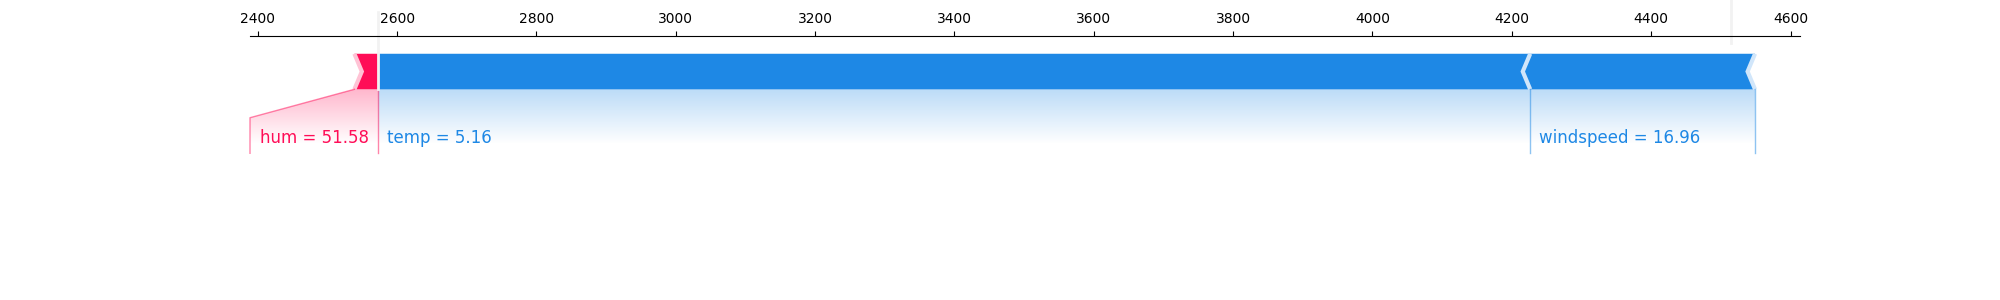
\includegraphics[width=\columnwidth]{figure_man/exSHAP.png}
%\end{figure}
%\end{frame}

\begin{frame}{Kernel SHAP - In 5 Steps}

\textbf{Definition:} A kernel-based, model-agnostic method to compute Shapley values via local surrogate models (e.g. linear model)\\
\vspace{1cm}
\begin{enumerate}
    \item Sample coalition vectors  \(\zv'\!\in\!\{0,1\}^p\)
    %\begin{onlyenv}<1>
   % $$z_{k}^{\prime} \in\{0,1\}^{M}, \quad k \in\{1, \ldots, K\}$$
    %\end{onlyenv}
    
    \item Map coalition vectors to original feature space and predict
    %Transfer coalitions into feature space \& get predictions by applying ML model
    
 %   \begin{onlyenv}<2>
  %  $$\hat{f}: \hat{f}\left(h_{x}\left(z_{k}^{\prime}\right)\right)$$
   % \end{onlyenv}
    
    \item Compute kernel weights for surrogate model
 %   \begin{onlyenv}<3>
 %   $$\pi_{x}\left(z^{\prime}\right)=\frac{(M-1)}{\left(\begin{array}{c} M \\\left|z^{\prime}\right|\end{array}\right)\left|z^{\prime}\right|\left(M-\left|z^{\prime}\right|\right)}$$
 %   \end{onlyenv}
    
    \item Fit a weighted linear model 
  %  \begin{onlyenv}<4>
  %  $$L\left(\hat{f}, g, \pi_{x}\right)=\sum_{z^{\prime} \in Z}\left[\hat{f}\left(h_{x}\left(z^{\prime}\right)\right)-g\left(z^{\prime}\right)\right]^{2} \pi_{x}\left(z^{\prime}\right)$$
  %  \end{onlyenv}

    \item Return Shapley values
%    \begin{onlyenv}<5>
%    $$(\phi_1, \ldots, \phi_M)$$
%    \end{onlyenv}
    
    
\end{enumerate}

\end{frame}



% \begin{frame}{Kernel SHAP in 5 Steps}

% \textbf{Goal:} Estimate Shapley values for a fixed instance \(\xv\) without model restrictions.

% \medskip
% \begin{enumerate}
%   \item \textbf{Sample coalitions}  
%         Draw \(K\) binary masks  
%         \(\zv'^{(k)}\!\in\!\{0,1\}^p\) (\(k=1,\dots,K\)); each mask marks a subset of “known” features.

%   \item \textbf{Create coalition inputs \& predict}  
%         Build \(\tilde{\xv}^{(k)}\) by  
%         \(\tilde{x}^{(k)}_j = x_j\) if \(z'^{(k)}_j=1\); otherwise impute.  
%         Evaluate the model: \(y^{(k)} = \fh\!\bigl(\tilde{\xv}^{(k)}\bigr)\).

%   \item \textbf{Assign kernel weights}  
%         \[
%           \pi_x(\zv') = \frac{p-1}{\binom{p}{|\zv'|}\,|\zv'|\,(p-|\zv'|)}
%         \]

%   \item \textbf{Fit weighted surrogate}  
%         Weighted least squares for  
%         \(g(\zv') = \phi_0 + \sum_{j=1}^p \phi_j z'_j\):
%         \[
%           \min_{\phi}\sum_{k=1}^K \bigl[y^{(k)} - g(\zv'^{(k)})\bigr]^2\,\pi_x(\zv'^{(k)})
%         \]

%   \item \textbf{Return Shapley estimates}  
%         Coefficients \(\phi_j(\xv)\) (and \(\phi_0\)) are the Kernel-SHAP attributions.
% \end{enumerate}

% \end{frame}


\begin{frame}{Kernel SHAP - In 5 Steps}


\textbf{Step 1: Sample coalition vectors}
\begin{itemize}
    \item Sample K coalitions from the simplified (binary) feature space
    $$\mathbf{z}^{\prime (k)} \in\{0,1\}^{p}, \quad k \in\{1, \ldots, K\}$$
    \item \( \mathbf{z}^{\prime (k)} \in \{0,1\}^p \) indicates which features are present in  \( k \)-th coalition
  \item To evaluate the model on each coalition, we must map \( \mathbf{z}^{\prime (k)} \) to original space %a full feature vector in the 
  
    \item Example ($\xv = (51.6, 5.1, 17.0)$) $\Rightarrow$ $2^p = 2^3 = 8$ coalitions (without sampling)
    %For our simple example, we have in total $2^p = 2^3 = 8$ coalitions (without sampling)
\end{itemize}


\begin{tikzpicture}
\fontsize{8}{12}

\node (tab1) {%
\begin{tabular}{l |ccc}
  \( \mathbf{z}^{(k)} \) & hum & temp & ws \\
  \hline
  \( \mathbf{z}^{(1)} \) & ? & ? & ? \\
  \( \mathbf{z}^{(2)} \) & 51.6 & ? & ? \\
  \( \mathbf{z}^{(3)} \) & ? & 5.1 & ? \\
  \( \mathbf{z}^{(4)} \) & ? & ? & 17.0 \\
  \( \mathbf{z}^{(5)} \) & 51.6 & 5.1 & ? \\
  \( \mathbf{z}^{(6)} \) & ? & 5.1 & 17.0 \\
  \( \mathbf{z}^{(7)} \) & 51.6 & ? & 17.0 \\
  \( \mathbf{z}^{(8)} \) & 51.6 & 5.1 & 17.0 \\
\end{tabular}};

\node [left=of tab1] (tab2) {%
  \begin{tabular}{l |c|ccc}
  Coalition & \( \mathbf{z}^{\prime(k)} \) & hum & temp & ws \\
  \hline
  \( \varnothing \) & \( \mathbf{z}^{\prime(1)} \) & 0 & 0 & 0 \\
  hum & \( \mathbf{z}^{\prime(2)} \) & 1 & 0 & 0 \\
  temp & \( \mathbf{z}^{\prime(3)} \) & 0 & 1 & 0 \\
  ws & \( \mathbf{z}^{\prime(4)} \) & 0 & 0 & 1 \\
  hum, temp & \( \mathbf{z}^{\prime(5)} \) & 1 & 1 & 0 \\
  temp, ws & \( \mathbf{z}^{\prime(6)} \) & 0 & 1 & 1 \\
  hum, ws & \( \mathbf{z}^{\prime(7)} \) & 1 & 0 & 1 \\
  hum, temp, ws & \( \mathbf{z}^{\prime(8)} \) & 1 & 1 & 1 \\
  \end{tabular}};

\draw[->] (tab2.north) to[out=10,in=170] node[below]{Map to original feature space} (tab1.north);
\end{tikzpicture}


\end{frame}




\begin{frame}{Kernel SHAP – In 5 Steps}

\textbf{Step 2: Map coalition vectors to original feature space and predict}

\begin{itemize}
  \item Define mapping \( h_{\xv, \xv'} : \{0,1\}^p \rightarrow \mathbb{R}^p \), where:
  $
  \left(h_{\xv, \xv'}(\mathbf{z}^{\prime})\right)_j =
  \begin{cases}
    x_j & \text{if } z_j^{\prime} = 1 \\
    x_j^\prime & \text{if } z_j^{\prime} = 0
  \end{cases}
  $
  \item Construct $\zv = h_{\xv, \xv'}(\mathbf{z}')$ where present features take their values from \( \xv \) and absent features are imputed with values from a \textcolor{orange}{random background sample \( \xv' = (64.3, 28.0, 14.5)\)}
  %\item Repeat with multiple background samples to approximate marginal/conditional expectations over the absent features (example below without repetitions)
  \item Evaluate the model on each constructed vector: $\hat{f} = \hat{f}(h_{\xv, \xv'}(\mathbf{z}^{\prime(k)}))$
\end{itemize}

\medskip

\begin{tikzpicture}
\fontsize{8}{12}

\node (tab1) {%
  \begin{tabular}{l |ccc | c}
  \( \mathbf{z}^{(k)} \) & hum & temp & ws & \( \hat{f}(h_{\xv}(\mathbf{z}^{\prime(k)})) \) \\
  \hline
  \( \mathbf{z}^{(1)} \) & \textcolor{orange}{64.3} & \textcolor{orange}{28.0} & \textcolor{orange}{14.5} & 6211 \\
  \( \mathbf{z}^{(2)} \) & 51.6 & \textcolor{orange}{28.0} & \textcolor{orange}{14.5} & 5586 \\
  \( \mathbf{z}^{(3)} \) & \textcolor{orange}{64.3} & 5.1 & \textcolor{orange}{14.5} & 3295 \\
  \( \mathbf{z}^{(4)} \) & \textcolor{orange}{64.3} & \textcolor{orange}{28.0} & 17.0 & 5762 \\
  \( \mathbf{z}^{(5)} \) & 51.6 & 5.1 & \textcolor{orange}{14.5} & 2616 \\
  \( \mathbf{z}^{(6)} \) & \textcolor{orange}{64.3} & 5.1 & 17.0 & 2900 \\
  \( \mathbf{z}^{(7)} \) & 51.6 & \textcolor{orange}{28.0} & 17.0 & 5411 \\
  \( \mathbf{z}^{(8)} \) & 51.6 & 5.1 & 17.0 & 2573 \\
  \end{tabular}};

\node [left=of tab1] (tab2) {%
  \begin{tabular}{l |c|ccc}
  Coalition & \( \mathbf{z}^{\prime(k)} \) & hum & temp & ws \\
  \hline
  \( \varnothing \) & \( \mathbf{z}^{\prime(1)} \) & 0 & 0 & 0 \\
  hum & \( \mathbf{z}^{\prime(2)} \) & 1 & 0 & 0 \\
  temp & \( \mathbf{z}^{\prime(3)} \) & 0 & 1 & 0 \\
  ws & \( \mathbf{z}^{\prime(4)} \) & 0 & 0 & 1 \\
  hum, temp & \( \mathbf{z}^{\prime(5)} \) & 1 & 1 & 0 \\
  temp, ws & \( \mathbf{z}^{\prime(6)} \) & 0 & 1 & 1 \\
  hum, ws & \( \mathbf{z}^{\prime(7)} \) & 1 & 0 & 1 \\
  hum, temp, ws & \( \mathbf{z}^{\prime(8)} \) & 1 & 1 & 1 \\
  \end{tabular}};

\draw[->] (tab2.north) to[out=10,in=170] node[below]{\( h_{\xv, \xv'}(\mathbf{z}^{\prime(k)}) \)} (tab1.north);
\end{tikzpicture}

\end{frame}


\begin{frame}{Kernel SHAP – In 5 Steps}

\textbf{Step 2: Map coalition vectors to original feature space and predict}

\medskip

\textbf{Fix coalition vector} \(\mathbf{z}'=(1,0,0)\); draw multiple \textcolor{orange}{background samples $\xv'^{(1)}, \dots, \xv'^{(B)}$}\\
\(\;\Rightarrow\) keep \textbf{hum}, replace \textbf{temp} and \textbf{ws} by draws from the background data.

\begin{table}\centering\small
\begin{tabular}{c|ccc|c}
Sample \(b\) & hum (from \(\xv\)) & temp (from $\xv'^{(b)}$) & ws (from $\xv'^{(b)}$)  & \(\hat{f}(h_{\xv, \xv'^{(b)}}(\mathbf{z}'))\) \\
\hline
1 & 51.6 & \textcolor{orange}{28.0} & \textcolor{orange}{14.5} & 4635 \\
2 & 51.6 & \textcolor{orange}{5.1} & \textcolor{orange}{14.5} & 3295 \\
3 & 51.6 & \textcolor{orange}{28.0} & \textcolor{orange}{17.0} & 5586 \\
$\vdots$ & \multicolumn{3}{c}{$\cdots$} & $\cdots$ \\
\end{tabular}
\end{table}

% \[
% \textstyle
% \overbrace{\frac{1}{B}\sum_{b=1}^{B}\hat{f}(h_{\xv, \xv'^{(b)}}(\mathbf{z}'))}^{\text{Monte-Carlo average}}
% \;\;\longrightarrow\;\;
% \mathbb{E}_{\mathbf{X}_{-S}}\bigl[f(\mathbf{x}_S,\mathbf{X}_{-S})\bigr]
% \]

\begin{itemize}
  \item Typically, many background samples $\xv'^{(1)}, \dots, \xv'^{(B)}$ are used to approximate the marginal expectation required for KernelSHAP via Monte-Carlo average:
  $$ \textstyle \mathbb{E}_{\mathbf{X}_{-S}}\bigl[f(\mathbf{x}_S,\mathbf{X}_{-S})\bigr] \approx
\frac{1}{B}\sum_{b=1}^{B}\hat{f}(h_{\xv, \xv'^{(b)}}(\mathbf{z}'))$$
\item Background samples \( \xv'^{(b)} \) are drawn from:
\begin{itemize}
  \item Conditional distribution \( \xv'^{(b)} \sim P_{\mathbf{X} \mid \mathbf{X}_S = \mathbf{x}_S} \) $\leadsto$ \textbf{Observational SHAP} 
  \item Marginal distribution \( \xv'^{(b)} \sim P_{\mathbf{X}} \) $\leadsto$  \textbf{Interventional SHAP}
\end{itemize}

\item The same procedure applies to every other coalition vector \(\mathbf{z}'^{(k)}\).
\end{itemize}

\end{frame}












% \begin{frame}{Kernel SHAP - In 5 Steps}


% \textbf{Step 2: Map coalition vectors to original feature space and predict}
% \begin{itemize}
%    % \item $$\hat{f}: \hat{f}\left(h_{x}\left(z_{k}^{\prime}\right)\right)$$
%    \item $\mathbf{z}^{\prime (k)}$ is 1 if features are are part of the $k$-th coalition, 0 if they are absent
%    \item To calculate predictions for these coalitions, we need to define a function which maps the binary feature space back to the original feature space
% \end{itemize}


% \begin{tikzpicture}
% \centering

% \fontsize{8}{12}

% \node (tab1) {%
%        \begin{tabular}{l |cccc}
%   $\xv^{coalition}$ &  hum & temp & ws \\
%   \hline 
%   $\xv^{\{\varnothing\}}$ & $\varnothing$ & $\varnothing$ &$\varnothing$  \\
%    $\xv^{\{hum\}}$ & 51.6 & $\varnothing$ & $\varnothing$  \\
%     $\xv^{\{temp\}}$ & $\varnothing$ & 5.1 & $\varnothing$  \\
%      $\xv^{\{ws\}}$ & $\varnothing$ & $\varnothing$ & 17.0  \\
%      $\xv^{\{hum, temp\}}$ & 51.6 & 5.1 & $\varnothing$  \\
%      $\xv^{\{temp, ws\}}$ &$\varnothing$ & 5.1 & 17.0  \\
%      $\xv^{\{hum, ws\}}$ & 51.6 & $\varnothing$ & 17.0  \\
%   $\xv^{\{hum, temp, ws\}}$ &51.6 & 5.1 & 17.0   \\
  
 
%   \end{tabular}};

% \node [left=of tab1] (tab2) {%
%      \begin{tabular}{l |c|ccc}
%   Coalition & $\mathbf{z}^{\prime (k)}$ &  hum & temp & ws \\
%   \hline 
%   $\varnothing$ & $\mathbf{z}^{\prime (1)}$ & 0 & 0 & 0  \\
%   hum & $\mathbf{z}^{\prime (2)}$ & 1 & 0 & 0  \\
%   temp &  $\mathbf{z}^{\prime (3)}$ & 0 & 1 & 0  \\
%   ws &   $\mathbf{z}^{\prime (4)}$ & 0 & 0 & 1  \\
%   hum, temp & $\mathbf{z}^{\prime (5)}$ & 1 & 1 & 0  \\
%   temp, ws & $\mathbf{z}^{\prime (6)}$ & 0 & 1 & 1  \\
%   hum, ws &   $\mathbf{z}^{\prime (7)}$ & 1 & 0 & 1  \\
%   hum, temp, ws & $\mathbf{z}^{\prime (8)}$ & 1 & 1 & 1  \\
   
 
%   \end{tabular}};
% \draw[->]
% (tab2.north) to[out=10,in=170] node[below]{} (tab1.north) ;
% \end{tikzpicture}

% \end{frame}


% \begin{frame}{Kernel SHAP - In 5 Steps}


% \textbf{Step 2: Map coalition vectors to original feature space and predict}
% \begin{itemize}
%    % \item $$\hat{f}: \hat{f}\left(h_{x}\left(z_{k}^{\prime}\right)\right)$$
%     \item Define 
% $h_x\left(\mathbf{z}^{\prime (k)}\right)=\mathbf{z}^{(k)} \text { where } h_x:\{0,1\}^{p} \rightarrow \R^{p}$
%  maps 1’s to feature values of observation $\xv$ for features part of the $k$-th coalition and 0's to feature values of a \color{orange}{randomly sampled observation} \color{black}for features absent in the $k$-th coalition
%   % \item Absent feature values are replaced by feature values of a \color{orange}{random observation} \color{black} of the dataset (permuted) $\leadsto$ permute feature values several times
%   (feature values are permuted multiple times) 
%    \item Predict with ML model on this dataset $\hat{f}: \hat{f}\left(h_{x}\left(\mathbf{z}^{\prime (k)}\right)\right)$
% \end{itemize}


% \begin{tikzpicture}
% \centering

% \fontsize{7}{12}

% \node (tab1) {%
%        \begin{tabular}{l |ccc | c}
%   $\mathbf{z}^{(k)}$ &  hum & temp & ws & $\hat{f}\left(h_{x}\left(\mathbf{z}^{\prime (k)}\right)\right)$\\
%   \hline 
%   $\mathbf{z}^{(1)}$ & \color{orange}{64.3} & \color{orange}{28.0} & \color{orange}{14.5} & 6211 \\
%    $\mathbf{z}^{(2)}$ & 51.6 & \color{orange}{28.0} & \color{orange}{14.5} & 5586  \\
%     $\mathbf{z}^{(3)}$ & \color{orange}{64.3} & 5.1 & \color{orange}{14.5}  & 3295\\
%      $\mathbf{z}^{(4)}$ & \color{orange}{64.3} & \color{orange}{28.0} & 17.0 &5762 \\
%      $\mathbf{z}^{(5)}$ & 51.6 & 5.1 & \color{orange}{14.5}  & 2616\\
%      $\mathbf{z}^{(6)}$ &\color{orange}{64.3} & 5.1 & 17.0  & 2900\\
%      $\mathbf{z}^{(7)}$ & 51.6 & \color{orange}{28.0} & 17.0 & 5411 \\
%   $\mathbf{z}^{(8)}$ &51.6 & 5.1 & 17.0 & 2573  \\
  
 
%   \end{tabular}};

% \node [left=of tab1] (tab2) {%
%      \begin{tabular}{l |c|ccc}
%   Coalition & $\mathbf{z}^{\prime (k)}$ &  hum & temp & ws \\
%   \hline 
%   $\varnothing$ & $\mathbf{z}^{\prime (1)}$ & 0 & 0 & 0  \\
%   hum & $\mathbf{z}^{\prime (2)}$ & 1 & 0 & 0  \\
%   temp &  $\mathbf{z}^{\prime (3)}$ & 0 & 1 & 0  \\
%   ws &   $\mathbf{z}^{\prime (4)}$ & 0 & 0 & 1  \\
%   hum, temp & $\mathbf{z}^{\prime (5)}$ & 1 & 1 & 0  \\
%   temp, ws & $\mathbf{z}^{\prime (6)}$ & 0 & 1 & 1  \\
%   hum, ws &   $\mathbf{z}^{\prime (7)}$ & 1 & 0 & 1  \\
%   hum, temp, ws & $\mathbf{z}^{\prime (8)}$ & 1 & 1 & 1  \\
  
%   \end{tabular}};
% \draw[->]
% (tab2.north) to[out=10,in=170] node[below]{$h_x(\mathbf{z}^{\prime (k)})$} (tab1.north) ;
% \end{tikzpicture}

% \end{frame}

\begin{frame}{Kernel shap - in 5 steps}
\textbf{Step 3: Compute kernel weights for surrogate model}\\\medskip
%\textbf{Intuition}: We learn most about individual features if we can study their effects in isolation or at maximal interaction:
%Small coalitions (few 1’s) and large coalitions (i.e. many 1’s) get the largest weights\\NB: the figure is independent from the running example

\begin{onlyenv}<1>
\textbf{Intuition:}  
We learn most about a feature’s effect when (recall multinomial coefficient in Shapley value's set definition):
\begin{itemize}
  \item it appears \textbf{in isolation} (small coalition), or
  \item in \textbf{near-complete context} (large coalition).
\end{itemize}
\(\Rightarrow\) SHAP assigns highest weights to very small and very large coalitions.

\medskip
\textbf{Note:} The figure below is illustrative and not tied to the running example.

\begin{figure}
    \centering
    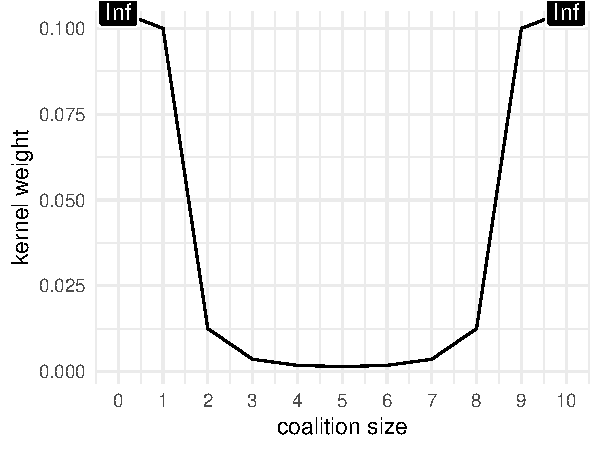
\includegraphics[width=0.5\columnwidth]{figure_man/kernel-weights.pdf}
    %\caption{Examplary dependence between kernel weights and coalition size for a data set p = 10 features}   
\end{figure}
\end{onlyenv}


\begin{onlyenv}<2>
\vspace{1cm}
\begin{exampleblock}{}
\[
\tikzmark{pi}\pi_{x}\left(\mathbf{z}^{\prime (k)}\right)=\frac{(
\tikzmark{M}p-1)}{\left(\begin{array}{c} p \\\left|\mathbf{z}^{\prime (k)}\right|\end{array}\right)\left|
\tikzmark{z}\mathbf{z}^{\prime (k)}\right|\left(p-\left|\mathbf{z}^{\prime (k)}\right|\right)}
\]
\begin{tikzpicture}[
  remember picture,
  overlay,
  expl/.style={draw=blue,fill=white,rounded corners,text width=4cm},
  arrow/.style={blue,ultra thick,->,>=latex}
]
\node[expl] 
  (piex) 
  at (2,2.5cm)
  {$\pi_x(\mathbf{z}^{\prime (k)})$: kernel weight for coalition $\mathbf{z}^{\prime (k)}$};
\node[expl] 
  (Mex) 
  at (8,3cm)
  {$p$: Number of features in $\xv$};
\node[expl] 
  (zex) 
  at (6,-1cm)
  {$\mid \mathbf{z}^{\prime (k)}\mid$: coalition size / sum of 1s in $\mathbf{z}^{\prime (k)}$};
\draw[arrow]
  (piex.south) to[out=270,in=135] ([xshift= 0.5ex, yshift=2ex]{pic cs:pi}); 
\draw[arrow]
  (Mex.south) to[out=270,in=90] ([xshift= 0.5ex, yshift=2ex]{pic cs:M}); 
\draw[arrow]
  (zex.north) to[out=90,in=250] ([xshift= 0.5ex, yshift=-1ex]{pic cs:z}); 
\end{tikzpicture}
\end{exampleblock}

\vspace{50pt}

\textbf{Note:} Weights differ from multinomial coefficient in the Shapley value set-definiton but are constructed to yield the same Shapley values via weighted linear regression.
%While this expression does not directly match the multinomial coefficient of Shapley value set definition, it is derived to produce the same weighted average over marginal contributions when using these weights in a weighted linear regression. 
\citebutton{see shapley\_kernel\_proof.pdf}{https://proceedings.neurips.cc/paper/2017/file/8a20a8621978632d76c43dfd28b67767-Supplemental.zip}
\end{onlyenv}


% \begin{onlyenv}<3>

% $$\pi_{x}\left(z^{\prime}\right)=\frac{(M-1)}{\left(\begin{array}{c} M \\\left|z^{\prime}\right|\end{array}\right)\left|z^{\prime}\right|\left(M-\left|z^{\prime}\right|\right)}$$

% \begin{itemize}
%     \item If a coalition consists of a single feature, we can learn about this feature’s isolated main effect on the prediction
%     \item If a coalition consists of all but one feature, we can learn about this feature’s total effect (main effect plus feature interactions)
%     \item If a coalition consists of half the features, we learn little about an individual feature’s contribution, as there are many possible coalitions with half of the features
% \end{itemize}
% \end{onlyenv}

% \begin{onlyenv}<4>
% \vspace{1cm}
% \textbf{Limited Budget $K$}: Can we be a bit smarter about the sampling of coalitions, than just randomly drawing?
% \begin{itemize}
%     \item The smallest and largest coalitions take up most of the weight\\ We get better Shapley value estimates by using some of the sampling budget K to include these high-weight coalitions
%     \item We start with all possible coalitions with 1 and M-1 features, which makes 2 times M coalitions in total\\ When we have enough budget left (current budget is K - 2M), we can include coalitions with 2 features and with M-2 features and so on.
%     \item From the remaining coalition sizes, we sample with readjusted weights
% \end{itemize}
% \end{onlyenv}
  
\end{frame}


\begin{frame}{Kernel shap - in 5 steps}
\textbf{Step 3: Compute kernel weights for surrogate model}\\\medskip

\only<1>{
%\textbf{Purpose}: to include this knowledge in the local surrogate model (linear regression), we calculate weights for each coalition which are the observations of the linear regression
\textbf{Purpose:} Assign observation weights $\pi_{x}\left(\mathbf{z}^{\prime}\right)$ to each coalition vector $\zv'$ when solving the local surrogate (weighted linear regression), e.g.:
%Assign weights to coalition vectors when fitting the local surrogate (linear regression) to account for their "importance"
$$\pi_{x}\left(\mathbf{z}^{\prime}\right)=\frac{(p-1)}{\left(\begin{array}{c} p \\|\mathbf{z}^{\prime}|\end{array}\right)|\mathbf{z}^{\prime}|(p-|\mathbf{z}^{\prime}|)} \leadsto \pi_x\left(\mathbf{z}^{\prime} = (1,0,0)\right)=\frac{(3-1)}{\left(\begin{array}{c} 3 \\1\end{array}\right)1\left(3-1\right)} = \frac{1}{3}$$
}


\only<2>{
\begin{itemize}
    \item For $p>3$ features, the finite weights are all 0.33 as every shown coalition has the same size ($|S|=1$ and $|-S|=2$ and vice versa for $p=3$).
    \item In general (when $p>3$), weights vary with coalition size.
    \item Empty and full coalitions receive weight $\infty$ (division-by-zero term)\\
    $\leadsto$ These coalition vectors are not used as observations for the linear regression\\
    $\leadsto$ Instead constraints are used to ensure \emph{local accuracy} and \emph{missingness}
\end{itemize}
% $\leadsto$ all the finite weights being equal to the same value (0.33) is the result of coalition size being equal to 3. In general the weight distribution is not uniform. 
% \\$\leadsto$ weights for empty and full set are infinity (since they result in division by 0 when calculating $\pi_{x}\left(\mathbf{z}^{\prime}\right)$) and not used as observations for the linear regression\\ $\leadsto$ instead constraints are used such that properties (local accuracy and missingness) are satisfied
}

\begin{table}[]
    \centering
        \begin{tabular}{l |c|ccc|c}
 Coalition & $\mathbf{z}^{\prime (k)}$ &  hum & temp & ws & weight $\pi_{x}\left(\mathbf{z}^{\prime}\right)$\\
  \hline 
  $\varnothing$ & $\mathbf{z}^{\prime (1)}$ & 0 & 0 & 0 & $\infty$ \\
  hum & $\mathbf{z}^{\prime (2)}$ & 1 & 0 & 0 & 0.33 \\
  temp &  $\mathbf{z}^{\prime (3)}$ & 0 & 1 & 0 & 0.33 \\
  ws &   $\mathbf{z}^{\prime (4)}$ & 0 & 0 & 1 & 0.33  \\
  hum, temp & $\mathbf{z}^{\prime (5)}$ & 1 & 1 & 0 & 0.33 \\
  temp, ws & $\mathbf{z}^{\prime (6)}$ & 0 & 1 & 1 & 0.33 \\
  hum, ws &   $\mathbf{z}^{\prime (7)}$ & 1 & 0 & 1 & 0.33 \\
  hum, temp, ws & $\mathbf{z}^{\prime (8)}$ & 1 & 1 & 1 & $\infty$ \\
  
 
  \end{tabular}
\end{table}
% \medskip

  
\end{frame}

%\begin{frame}{Coalition Mapping}
%We define a coalition $z^{\prime}$, by describing a function 

%$$
%h\left(z^{\prime}\right)=z \text { where } h:\{0,1\}^{M} \rightarrow \mathbb{R}^{p}
%$$


%\begin{onlyenv}<1>
%\vspace{1cm}
%\begin{itemize}
%    \item Coalition $z^{\prime} \in \{0, 1\}^M$ is the  vector, indicating if feature $j$ contributes to the prediction 
%    \item $h(\cdot)$ represent a function that maps 1’s to the corresponding value from the observation x that we want to explain: $h(\cdot)$ connects our coalition vector to the underlying data 
%\end{itemize}
%\end{onlyenv}

%\begin{onlyenv}<2->
%\begin{tikzpicture}
%\centering

%\node<2> (tab1) {%
%  \begin{tabular}{l |cccc}
%  observation & temp & hum & ws & yr\\
%  \hline 
%  $x_{ex}$ & 24.7 & 58.5 & 13.96 & 2011\\
 % \\
 % \\
  %\end{tabular}};
%\node<3-> (tab1) {%
%  \begin{tabular}{l |cccc}
%  observation & temp & hum & ws & yr\\
%  \hline 
%  $x_{ex}$ & 24.7 & 58.5 & 13.96 & 2011\\
%  $z_{temp, yr}$ & 24.7 & $\varnothing$ & $\varnothing$ & 2011\\
%  $z_{yr}$ & $\varnothing$ & $\varnothing$ & $\varnothing$ & 2011\\
%  \end{tabular}};
%\node<2> [left=of tab1] (tab2) {%
%  \begin{tabular}{l |cccc}
%  Coalition & temp & hum & ws & yr\\
%  \hline 
%  $x^{\prime}$ & 1 & 1 & 1 & 1 \\
%  \\
%  \\
%  \end{tabular}};
%\node<3-> [left=of tab1] (tab2) {%
%  \begin{tabular}{l |cccc}
%  Coalition & temp & hum & ws & yr\\
%  \hline 
%  $x^{\prime}$ & 1 & 1 & 1 & 1 \\
%  $z^{\prime}_{temp, yr}$ & 1 & 0 & 0 %& 1 \\
%  $z^{\prime}_{yr}$ & 0 & 0 & 0 & 1 %\\
%  \end{tabular}};
%\draw<2->[->]
%(tab2.north) to[out=30,in=150] node[below]{$h(\cdot)$} (tab1.north) ;
%\end{tikzpicture}
%\end{onlyenv}
%\begin{onlyenv}<3->
%\begin{itemize}
%    \item $h(\cdot)$ maps 1’s to the %corresponding value from the observation x that we want to explain
%    \item<4> it maps 0’s to the values of another observation that we sample from the data
%    \item<4>  we equate “feature value is absent” with “feature value is replaced by random feature value from data”
%\end{itemize}
%\end{onlyenv}
%\end{frame}


% \begin{frame}{Kernel shap - in 5 steps}
% \textbf{Step 4: Fit a weighted linear model}\\\medskip
% \textbf{Aim}: Estimate a weighted linear model with Shapley values being the coefficients $\phi_j$
% $$
% g\left(\mathbf{z}^{\prime (k)}\right)=
% \phi_{0}+\sum_{j=1}^{p}
%  \phi_{j} z_{j}^{\prime (k)} \only<2>{\leadsto g\left(\mathbf{z}^{\prime (k)}\right)=
% 4515 +
%  34 \cdot z_{1}^{\prime (k)} - 1654 \cdot z_{2}^{\prime (k)} - 323 \cdot z_{3}^{\prime (k)} }
% $$


% \only<1>{
% and minimize by WLS using the weights $\pi_{x}$ of step 3
%     $$L\left(\hat{f}, g, \pi_{x}\right)=\sum_{k = 1}^K\left[\hat{f}\left(h_{x}\left(\mathbf{z}^{\prime (k)}\right)\right)-g\left(\mathbf{z}^{\prime (k)}\right)\right]^{2} \pi_{x}\left(\mathbf{z}^{\prime (k)}\right)$$

% with $\phi_0 = \E(\fh)$ and $\phi_p = \fh(x) - \sum_{j=0}^{p-1} \phi_j$ we receive a $p-1$ dimensional linear regression problem
% }

% \only<2>{
% \begin{table}[]
%     \centering
%         \begin{tabular}{l |ccc|c|c}
%   $\mathbf{z}^{\prime (k)}$ &  hum & temp & ws & weight & $\fh$\\
%   \hline 
%    $\mathbf{z}^{\prime (2)}$ & 1 & 0 & 0 & 0.33 & 4635\\
%     $\mathbf{z}^{\prime (3)}$ & 0 & 1 & 0 & 0.33 & 3087\\
%      $\mathbf{z}^{\prime (4)}$ & 0 & 0 & 1 & 0.33 & 4359\\
%      $\mathbf{z}^{\prime (5)}$ & 1 & 1 & 0 & 0.33 & 3060\\
%      $\mathbf{z}^{\prime (6)}$ & 0 & 1 & 1 &0.33 & 2623\\
%      $\mathbf{z}^{\prime (7)}$ & 1 & 0 & 1 & 0.33 & 4450\\
%       \multicolumn{1}{c}{} & \multicolumn{3}{c}{\upbracefill}&\multicolumn{1}{c}{} &\multicolumn{1}{c}{\upbracefill}\\[-1ex]
%     \multicolumn{1}{c}{} & \multicolumn{3}{c}{$\scriptstyle input$}&\multicolumn{1}{c}{} &  \multicolumn{1}{c}{$\scriptstyle output$}\\
  
 
%   \end{tabular}
% \end{table}
% }


  
% \end{frame}





\begin{frame}{Kernel shap - in 5 steps}

\textbf{Step 4: Fit a weighted linear model}\\\medskip

\textbf{Goal} Estimate Shapley values \( \phi_j \) as coefficients of a local, weighted linear surrogate.
\[
\textstyle g(\mathbf{z}') \;=\; \phi_0 \;+\; \sum_{j=1}^{p} \phi_j z'_j
\]

\only<1>{
\textbf{Weighted least-squares objective}

\[
\textstyle
\min_{\phi}\;
\sum_{k=1}^{K}
\pi_x(\mathbf{z}'^{(k)})
\Bigl[
  \hat{f}\bigl(h_{\xv}(\mathbf{z}'^{(k)})\bigr)
  - g(\mathbf{z}'^{(k)})
\Bigr]^2
\]
Boundary coalitions ($\zv' = \mathbf{1}$ and $\zv'=\mathbf{0}$) enforce constraints on coefficients
\[
\textstyle 
\phi_0 = \mathbb{E}[\hat{f}(\mathbf{X})],
\qquad
\sum_{j=1}^{p} \phi_j = \hat{f}(\xv)-\phi_0 .
\]
}

%\medskip
\only<2>{
\textbf{Numeric illustration (\(p=3\))}

\[
g(\mathbf{z}')
= 4515
+ 34\,z'_1
-1654\,z'_2
-323\,z'_3
\]

\begin{table}\centering\small
\begin{tabular}{c |ccc|c|c|c}
\( \mathbf{z}' \) & hum & temp & ws & weight $\pi_{x}\left(\mathbf{z}^{\prime}\right)$ & \( \hat{f}( h_{\xv}(\mathbf{z}')) \) & \( g(\mathbf{z}') \) \\
\hline
\( (1,0,0) \) & 1 & 0 & 0 & 0.33 & 4635 & 4549 \\
\( (0,1,0) \) & 0 & 1 & 0 & 0.33 & 3087 & 2861 \\
\( (0,0,1) \) & 0 & 0 & 1 & 0.33 & 4359 & 4192 \\
\( (1,1,0) \) & 1 & 1 & 0 & 0.33 & 3060 & 2895 \\
\( (0,1,1) \) & 0 & 1 & 1 & 0.33 & 2623 & 2538 \\
\( (1,0,1) \) & 1 & 0 & 1 & 0.33 & 4450 & 4226 \\
\multicolumn{1}{c}{} & \multicolumn{3}{c}{\upbracefill}
  & \multicolumn{1}{c}{} &
  \multicolumn{1}{c}{\upbracefill} \\[-1ex]
\multicolumn{1}{c}{} & \multicolumn{3}{c}{\scriptsize inputs}
  & \multicolumn{1}{c}{} &
  \multicolumn{1}{c}{\scriptsize outputs} \\
\end{tabular}
\end{table}

The inputs and outputs are used to learn the weighted linear regression model.
}

\end{frame}


\begin{frame}{Kernel shap - in 5 steps}
\textbf{Step 5: Return SHAP values}\\\medskip
\textbf{Intuition}: Estimated Kernel SHAP values are equivalent to Shapley values 
\begin{align*}
g(\mathbf{z}^{\prime (8)}) &= \fh(h_x(\mathbf{z}^{\prime (8)}) ) = 4515 + 34 \cdot 1 - 1654 \cdot 1 - 323 \cdot 1\\&= \underbrace{\E(\fh)}_{\phi_0} + \phi_{hum} + \phi_{temp} + \phi_{ws} = \fh(\xv) = 2573
\end{align*}

\begin{figure}
    \centering
    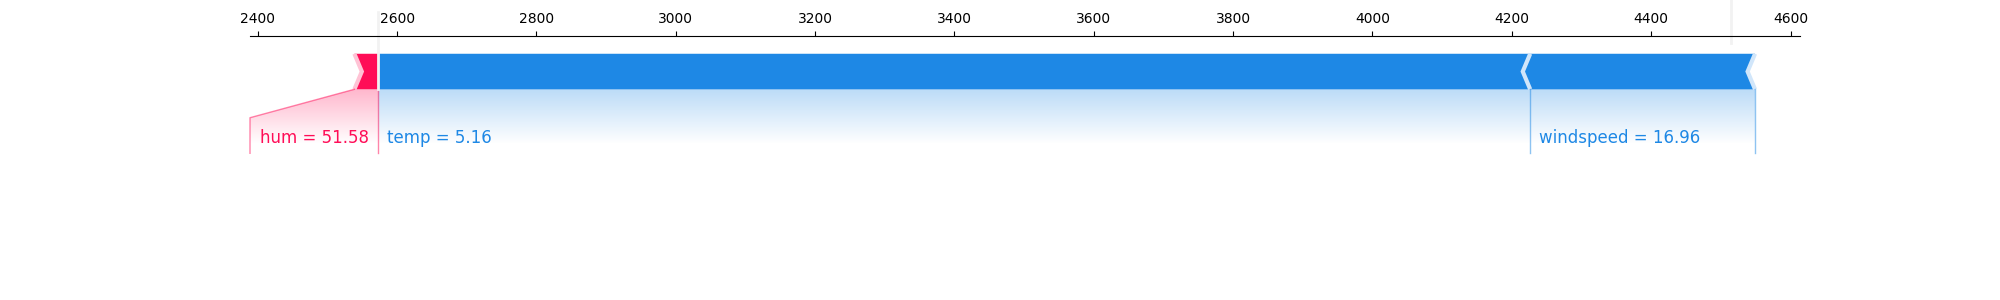
\includegraphics[width=\columnwidth]{figure_man/exSHAP.png}
    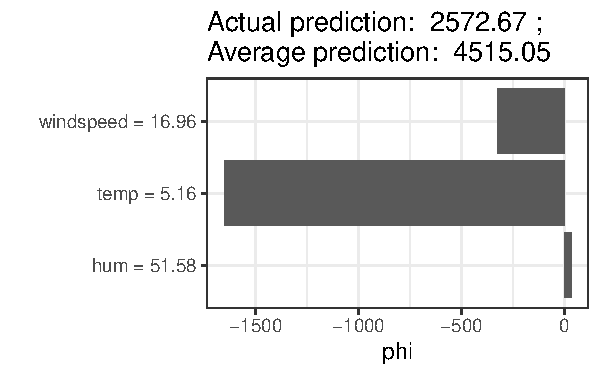
\includegraphics[trim={10 17 5 5},clip, width=0.4\linewidth]{figure/shapley2shap.pdf}
\end{figure}


\end{frame}
%\begin{frame}{Marginal Contribution}

%\begin{itemize}
%    \begin{onlyenv}<1>
%    \item Consider coalition $z^{\prime}$ as indicator function for our shapley values $\phi$
%    \end{onlyenv}
%    \begin{onlyenv}<2>
%    \item This connects the coalition vector $z^{\prime}$ to the respective marginal contribution
%    \end{onlyenv}
%    \begin{onlyenv}<3>
%    \item To estimate the marginal contribution, we can transfer the coalition to the data space by $h(z^{\prime})$
%    \end{onlyenv}
%    \begin{onlyenv}<4->
%    \item $\fh(h(z^{\prime}))$ connects the coalitions directly to the marginal distribution.
%    \end{onlyenv}
%\end{itemize}

%\vspace{1cm}

%\begin{tikzpicture}
%\centering

%\node<1-2> (tab1) {%
%  \begin{tabular}{l |cccc}
%  Coalition & temp & hum & ws & yr\\
%  \hline 
%  $x^{\prime}$ & 1 & 1 & 1 & 1 \\
%  $z^{\prime}_{temp, yr}$ & 1 & 0 & 0 & 1 \\
%  $z^{\prime}_{yr}$ & 0 & 0 & 0 & 1 \\
%  \end{tabular}};
%\node<2-> [right=of tab1] (tab2) {%
%\begin{tabular}{l | cccc}
%  & temp & hum & ws & yr\\
%  \hline 
%  $g(x^{\prime})$ & $\phi_{temp}$ + & $\phi_{hum}$ + & $\phi_{ws}$ + & $\phi_{yr}$ \\
%  $g(z^{\prime}_{temp, yr})$ & $\phi_{temp}$ + &  &  & $\phi_{yr}$\\
%   $g(z^{\prime}_{yr})$ & &  &  & $\phi_{yr}$ \\
%  \end{tabular}};
%\node<3-> [left=of tab2] (tab) {%
%  \begin{tabular}{l |cccc}
%  observation & temp & hum & ws & yr\\
%  \hline 
%  $x_{ex}$ & 24.7 & 58.5 & 13.96 & %2011\\
%  $z_{temp, yr}$ & 24.7 & %$\varnothing$ & $\varnothing$ & %2011\\
%  $z_{yr}$ & $\varnothing$ & %$\varnothing$ & $\varnothing$ & 2011\\
%  \end{tabular}};
%\draw<2>[->]
%(tab1.south) to[out=320,in=200] node[above]{$\sum \mathbb{I}_{[z^{\prime}_i == 1]} \phi_i$} (tab2.south) ;
%\draw<3->[->]
%(tab2.south) to[out=200,in=330] node[above]{$\fh(h(z^{\prime}))$} (tab1.south) ;
%\end{tikzpicture}

%\begin{onlyenv}<4>
%\begin{equation}
%\begin{array}{lllc}
  
%  g(x^{\prime}) &= \phi_{temp} + \phi_{hum} + \phi_{ws} + &\phi_{yr} &= 6825\\
%  g(z^{\prime}_{temp, yr}) &= \phi_{temp} + &\phi_{yr} &= 6134\\
%   g(z^{\prime}_{yr}) &= &\phi_{yr} &= 4325\\
%\end{array}
%\end{equation}
%\end{onlyenv}

%\begin{onlyenv}<5>
%\vspace{0.5cm}

%\textbf{Notice:}\\ We created a coalition data set $Z^{\prime}$ here by sampling multiple coalitions from observation $\xv$ that is evaluable with the prediction function $\fh$
%\end{onlyenv}

%\end{frame}



\endlecture
\end{document}
